\documentclass[11pt,a4paper]{article}

\usepackage[a4paper,margin=1in,footskip=0.25in]{geometry}
\usepackage{amsmath}
\usepackage{amssymb}
\usepackage{graphicx}
\usepackage{dcolumn}
\usepackage{bm}
\usepackage{cprotect}
\usepackage{spverbatim}

\usepackage{siunitx}

\usepackage[caption=false]{subfig}
\usepackage{printlen}
\usepackage{xspace}

\usepackage{fancyhdr}
\pagestyle{fancy}
\fancyhf{}
\rhead{Wannier 2022 Summer School}
\lhead{Giovanni Pizzi, Junfeng Qiao}
\cfoot{\thepage}

\usepackage{tabularx}
\usepackage{dcolumn}
\usepackage{booktabs}
\usepackage[inline]{enumitem}

\usepackage[cache=false]{minted}%

\usepackage{hyperref}
\usepackage[capitalize]{cleveref}

\usepackage[backend=biber,style=phys]{biblatex}
\addbibresource{main.bib}

\begin{document}

\definecolor{LightGray}{gray}{0.9}
\setminted{
  bgcolor=LightGray, }

\title{Hands-on:\\
  \textbf{Thermoelectric and electronic transport properties with Wannier90+BoltzWann}}

\author{Giovanni Pizzi \and Junfeng Qiao}

\date{20 May 2022}
\maketitle

\newcommand{\wan}{\texttt{Wannier90}\xspace}
\newcommand{\boltzwan}{\texttt{BoltzWann}\xspace}
\newcommand{\pwx}{\texttt{pw.x}\xspace}
\newcommand{\ptowx}{\textnormal{\texttt{pw2wannier90.x}}\xspace}
\newcommand{\wanx}{\textnormal{\texttt{wannier90.x}}\xspace}
\newcommand{\postwanx}{\textnormal{\texttt{postw90.x}}\xspace}

\section{Outline}

\begin{itemize}
  \item Obtain MLWFs for the valence and low-lying conduction states of silicon.
  \item Calculate the electrical conductivity, the Seebeck coefficient and the thermal
        conductivity in the constant relaxation time approximation using the \boltzwan
        module\cite{Pizzi2014,Pizzi2014a}.
\end{itemize}

\section{Input files \& executables}
\begin{itemize}
  \item{Directory: \texttt{wannier-tutorials/2022\_05\_Trieste/DAY5\_AM\_2\_BoltzWann/}}
  \item{Input Files}
  \begin{itemize}
    \item \texttt{Si.scf}: The \pwx input file for ground state
          calculation
    \item \texttt{Si.nscf}: The \pwx input file to obtain Bloch
          states on a uniform grid
    \item \texttt{Si.pw2wan}: Input file for \ptowx
    \item \texttt{Si.win}: The \wanx and \postwanx input file
  \end{itemize}
  \item Executables:
        \begin{itemize}
          \item \pwx, \ptowx, \wanx, and \postwanx
          \item Available in \texttt{/media/ictpuser/AiiDA/bin/}
        \end{itemize}
\end{itemize}

\section{Steps}
We will first run the standard Wannierization of silicon, then run the
\postwanx with \boltzwan related parameters added to the input file.
\begin{enumerate}
  \item Run \pwx to obtain the ground state of silicon
        \begin{minted}{bash}
pw.x < Si.scf > scf.out
\end{minted}

  \item Run \pwx to obtain the Bloch states on a uniform k-point grid.
        \begin{minted}{bash}
pw.x < Si.nscf > nscf.out
  \end{minted}

  \item Run \wanx to generate a list of the required overlaps (written into the
        \texttt{Si.nnkp} file).
        \begin{minted}{bash}
wannier90.x -pp Si
        \end{minted}

  \item Run \ptowx to compute the overlap between Bloch states and the projections for
        the starting guess (written in the \texttt{Si.mmn} and \texttt{Si.amn} files).
        \begin{minted}{bash}
pw2wannier90.x < Si.pw2wan > pw2wan.out
        \end{minted}

  \item Run \wanx to compute the MLWFs.
        \begin{minted}{bash}
wannier90.x Si
\end{minted}

        Inspect the output file \texttt{Si.wout} and check if the convergence was
        reached both in the disentanglement and in the Wannierization steps. You may
        also want to plot the Wannier functions and the interpolated band structure.

  \item Run \postwanx to calculate the transport coefficients.
        \begin{minted}{bash}
# serial execution
postw90.x Si
# or parallel execution with, e.g. 4 MPI processes
mpirun -np 4 postw90.x Si
\end{minted}
\end{enumerate}

\section{Analysis}
\begin{itemize}
\item Inspect the output file \texttt{Si.wpout}. It summarizes the main details of
the calculation (more details can be obtained by setting a larger value of the
\texttt{iprint} flag). Check if no warnings are issued. Note that if no special
flags are passed to \boltzwan, it assumes that the ab-initio calculation did
not include magnetization effects, and thus it sets to 2 the number of
electrons per state.

\item Note also that the value of the relaxation time $\tau$ = \SI{10}{fs} in the
example is set only as a representative value; note also that only the
electrical and thermal conductivity depend on $\tau$, while the Seebeck
coefficient is independent of $\tau$.

\item Using your favorite plotting program, plot the \texttt{Si\_boltzdos.dat} file
to inspect the DOS, e.g. with \texttt{gnuplot}, see \cref{fig:dos}.
\begin{minted}{gnuplot}
set xlabel 'E (eV)'
set ylabel 'DOS (ang^{-3})'
plot 'Si_boltzdos.dat' w l
\end{minted}
\begin{figure}[htb]
  \centering
  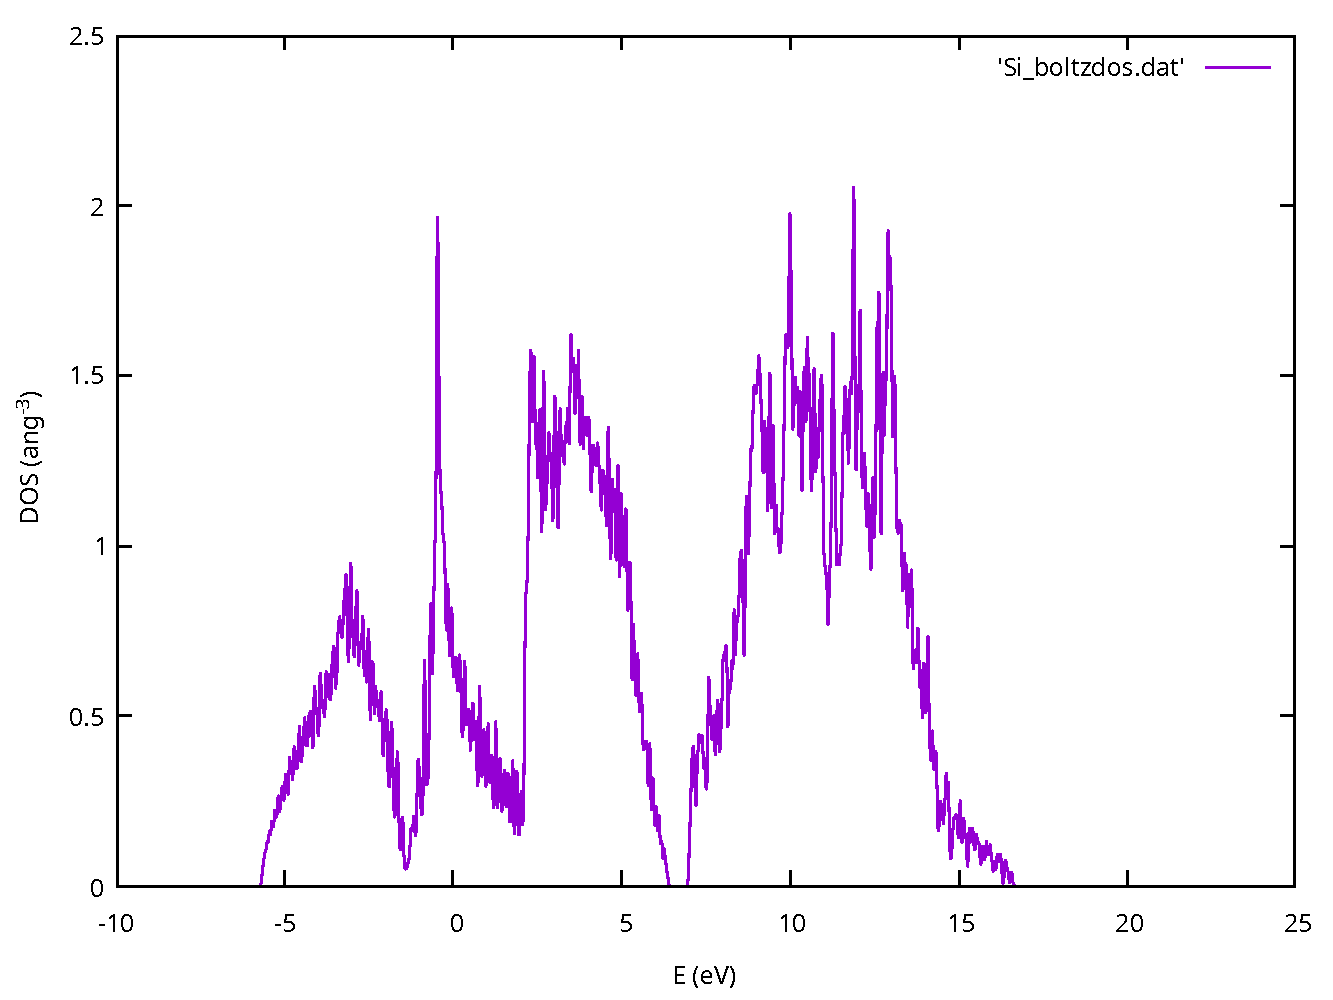
\includegraphics[width=.7\textwidth]{fig/dos.pdf}
  \caption{DOS of silicon using \boltzwan module.}
  \label{fig:dos}
\end{figure}

\item Using your favorite plotting program, plot columns 1 and 3 of the
\texttt{Si\_seebeck.dat} file to inspect the $S_{xx}$ component of the Seebeck
coefficient as a function of the chemical potential $\mu$, at $T$ =
\SI{300}{K}. For example, with \texttt{gnuplot}, see \cref{fig:seebeck}.
\begin{minted}{gnuplot}
set xlabel 'E (eV)'
set ylabel 'DOS (S_{xx} (V/K))'
plot 'Si_seebeck.dat' u 1:3 w l
\end{minted}
\begin{figure}[htb]
  \centering
  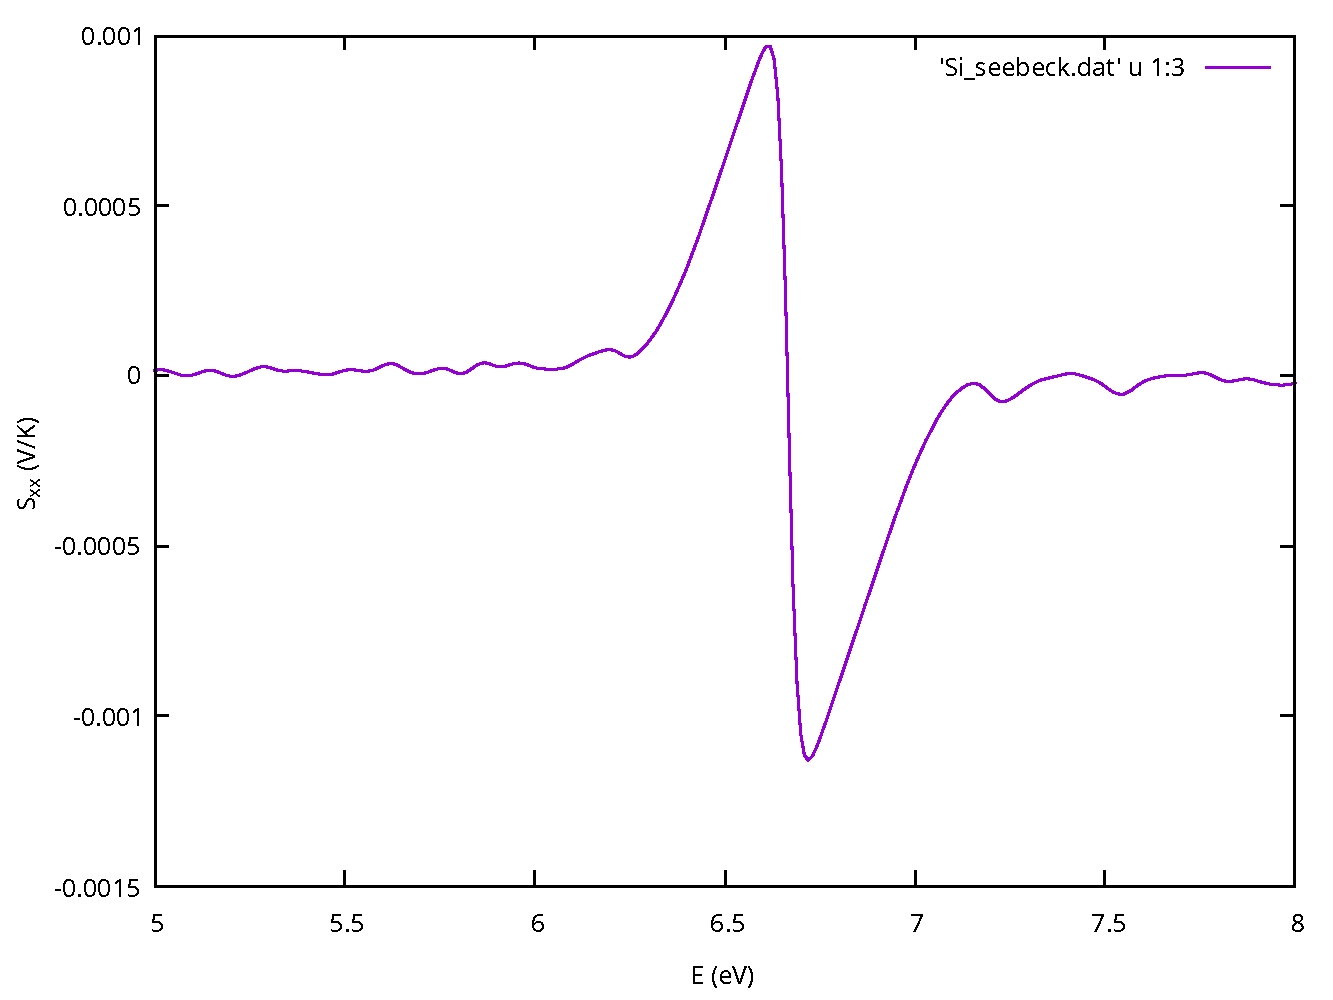
\includegraphics[width=.7\textwidth]{fig/seebeck.pdf}
  \caption{$S_{xx}$ of silicon using \boltzwan module.}
  \label{fig:seebeck}
\end{figure}
\end{itemize}

\subsection{Further ideas}

\begin{itemize}
  \item Change the interpolation to a $60\times 60\times 60$ mesh and run again
        \postwanx to check if the results for the transport properties are converged.

  \item Change the \texttt{Si.win} input file so that it calculates the transport
        coefficients for temperatures from \SIrange{300}{700}{K}, with steps of
        \SI{200}{K}. Rerun \postwanx and verify that the increase in execution time is
        neglibile (in fact, most of the time is spent to interpolate the band structure
        on the $k$ mesh).

        Plot the Seebeck coefficient for the three temperatures $T$ = \SI{300}{K}, $T$
        = \SI{500}{K} and $T$ = \SI{700}{K}. To do this, you have to filter the
        \texttt{Si\_seebeck.dat} to select only those lines where the second column is
        equal to the required temperature. A possible script to select the $S_{xx}$
        component of the Seebeck coefficient for $T$ = \SI{500}{K} using the
        \texttt{awk/gawk} command line program is the following:
        \begin{minted}{bash}
awk '{if ($2 == 500) {print $1, $3;}}' < Si_seebeck.dat \
    > Si_seebeck_xx_500K.dat
\end{minted}
        Then, you can plot columns 1 and 2 of the output file
        \verb#Si_seebeck_xx_500K.dat#.
  \item Try to calculate the Seebeck coefficient as a function of the temperature, for
        a $n-$doped sample with, e.g., $n$ = \SI{1e18}{cm^{-3}}. Note that to this aim,
        you need to calculate consistently the value $\mu(T)$ of the chemical potential
        as a function of the temperature, so as to reproduce the given value of $n$.
        Then, you have to write a small program/script to interpolate the output of
        \boltzwan, that you should have run on a suitable grid of $(\mu,T)$ points.
\end{itemize}

\printbibliography

\end{document}
